\chapter{Pattern GRASP}
\section{Definizione}
I pattern GRASP (General Responsibility Assignment Software Pattern) sono un insieme di \uline{principi fondamentali e linee guida} utilizzati nella \textbf{progettazione del software orientata agli oggetti} per supportare il progettista nell'assegnazione delle responsabilità a classi e oggetti.

\subsection{Approccio RDD}
Più che schemi di codice preconfezionati, i GRASP deniscono un approccio metodologico noto come \textbf{Responsability-Driven Design (Progettazione Guidata alla responsabilità)} formalizzando sotto forma di pattern le regole e le soluzioni idiomatiche applicate.

\subsection{Principi fondamentali}
\begin{itemize}
    \item \textbf{Focus sulle Responsabilità:}\\
    Nella progettazione a oggetti, i requisiti espressi nei casi d'uso vengono soddisfatti traducendoli in responsabilità per le classi del software.

    Tali responsabilità si dividono in 2 macro-categorie:
    \begin{itemize}
        \item \textbf{Responsabilità di FARE (Doing):} \uline{Come eseguire un'azione di business}, creare un altro oggetto o coordinare attività.
        \item \textbf{Responsabilità di CONOSCERE (Knowing):} Come la \uline{conoscenza dei propri dati privati incapsulati, delle relazioni o di elementi calcolabili}.
    \end{itemize}
    
    \item \textbf{Applicazione Dinamica:}\\
    Lo strumento principale in cui si applicano e si concretizzano i pattern GRASP è il disegno dei \textbf{diagrammi di interazione UML}.

    È proprio nel momento in cui si definiscono i messaggi scambiati tra gli oggetti che il progettista sceglie a quale entità assegnare una specifica funzione.
    \item \textbf{Obiettivo Qualificativo:}\\
    L'applicazione metodica di questi pattern mira a \uline{massimizzare metriche software essenziali}, riducendo l'impatto dei cambiamenti futuri e migliorando la manutenibilità.\\
    I due capisaldi di questo obiettivo sono il raggiungimento di un \textbf{accoppiamento basso}(Low Coupling) e di una \textbf{coesione alta}(High Cohesion)
\end{itemize}

\newpage
\subsection{Relazione tra gli elaborati}
\begin{figure}[H]
    \centering
\end{figure}

\section{Rappresentazione di un Pattern GRASP}
\begin{tabularx}{\textwidth}{@{} l X @{}}
\toprule
\textbf{Nome del pattern:} & \textbf{Information Expert} \\ \midrule
\textbf{Problema:}         & Qual è un principio di base con cui assegnare responsabilità agli oggetti? \\ \midrule
\textbf{Soluzione:}        & Assegna una responsabilità alla classe che ha le informazioni necessarie per soddisfarla. \\ 
\bottomrule
\end{tabularx}

\chapter{Pattern GRASP di base}
\section{Creator}
\subsection{Definizione}
\begin{table}[htbp]
    \renewcommand{\arraystretch}{1.8}
    \begin{tabularx}{\textwidth}{@{} p{2.8cm} X @{}}
        \hline
        Nome: & \textbf{Creator} \\
        \hline
        Problema: &  Chi crea un oggetto A?\\
        \hline
        Soluzione : &
        Assegna alla classe B la responsabilità di creare un'istanza della classe A se una delle seguenti condizioni è vera:
        \begin{itemize}
            \item B "contiene" o aggrega una composizione oggetti di tipo A
            \item B registra A
            \item B utilizza strettamente A
            \item B possiede i dati per l'inizializzazione di A
        \end{itemize} \\
        \hline
    \end{tabularx}
\end{table}

\subsection{Esempio diagramma delle classi}
\begin{figure}[H]
    \centering
    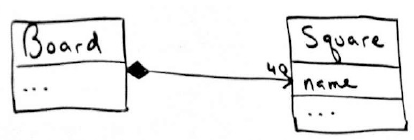
\includegraphics{Immagini/Schermata_20260712_123204.png}
\end{figure}
\subsection{Esempio diagramma di sequenza di stato}
\begin{figure}[H]
    \centering
    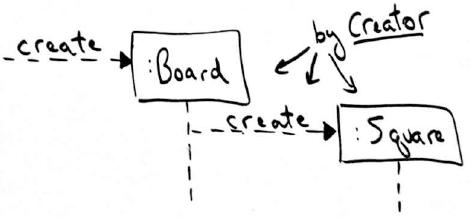
\includegraphics{Immagini/Schermata_20260712_123238.png}
\end{figure}

\newpage
\section{Information Expert}
\subsection{Definizione}
\begin{table}[htbp]
    \renewcommand{\arraystretch}{1.8}
    \begin{tabularx}{\textwidth}{@{} p{2.8cm} X @{}}
        \hline
        Nome: & \textbf{Information Expert} \\
        \hline
        Problema: &  Qual'è un principio di base per assegnare responsabilità agli oggetti\\
        \hline
        Soluzione : &
        Assegna una responsabilità alla classe che possiede le informazione necessarie per soddisfarla
        \\
        \hline
    \end{tabularx}
\end{table}

\subsection{Esempio diagramma delle classi}
\begin{figure}[H]
    \centering
    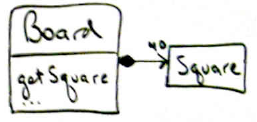
\includegraphics{Immagini/Schermata_20260712_123639.png}
\end{figure}
\subsection{Esempio diagramma di sequenza di stato}
\begin{figure}[H]
    \centering
    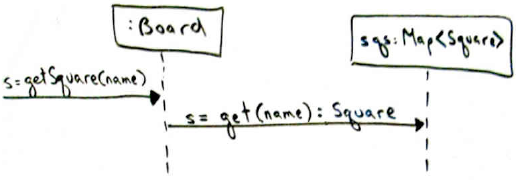
\includegraphics{Immagini/Schermata_20260712_123716.png}
\end{figure}

\newpage
\section{Low Coupling}
\subsection{Definizione}
\begin{table}[htbp]
    \renewcommand{\arraystretch}{1.8}
    \begin{tabularx}{\textwidth}{@{} p{2.8cm} X @{}}
        \hline
        Nome: & \textbf{Low Coupling} \\
        \hline
        Problema: &  Come ridurre l'impatto dei cambiamenti?\\
        \hline
        Soluzione : &
        Assegna le responsabilità in modo tale che l'accoppiamento (non necessario) rimanga basso. 

        Usa questo principio per valutare le alternative
        \\
        \hline
    \end{tabularx}
\end{table}
\subsection{Effetto di Information Expert}
Information Expert guida verso una scelta che sostiene Low Coupling
\begin{itemize}
    \item Expert chiede di trovare l'oggetto che possiede la maggior parte delle informazioni richieste per la responsabilità
    \item Se ingoriamo i consigli di Informatio Expert, l'accoppiamento complessivo è meggiore
    \begin{itemize}
        \item Ci sono più oggetti o informazioni che devono essere condivisi
    \end{itemize}
\end{itemize}

\subsection{Esempio di alto accoppiamento}
\begin{figure}[H]
    \centering
    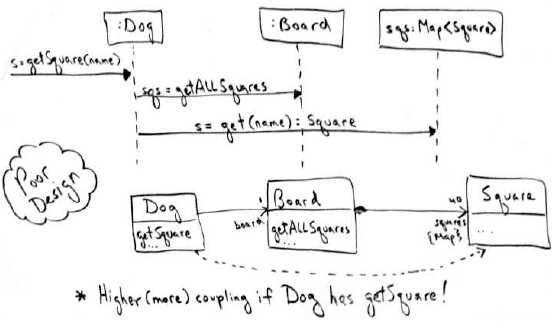
\includegraphics{Immagini/Schermata_20260712_183838.png}
\end{figure}

\newpage
\section{Controller}
\subsection{Definizione}
\begin{table}[htbp]
    \renewcommand{\arraystretch}{1.8}
    \begin{tabularx}{\textwidth}{@{} p{2.8cm} X @{}}
        \hline
        Nome: & \textbf{Controller} \\
        \hline
        Problema: &  Qual'è il primo oggetto oltre lo strato UI a ricevere e coordinare un'operazione di sistema\\
        \hline
        Soluzione : &
        Assegna la responsabilità a un oggetto che rappresenta una delle seguenti scelte:
        \begin{itemize}
            \item Rappresentare il "sistema" complessivo, un "oggetto radice", un dispositivo all'interno del quale viene eseguito il software, un punto d'accesso al software o un sottosistema principale (sono tutte varianti di un facade controller)
            \item Rappresenta uno scenario di un caso d'udo all'interno del quale si verifica l'operazione di sistema (un controller di caso d'uso o controller di session)
        \end{itemize}
        \\
        \hline
    \end{tabularx}
\end{table}

\subsection{Possibili approcci}
\begin{figure}[H]
    \centering
    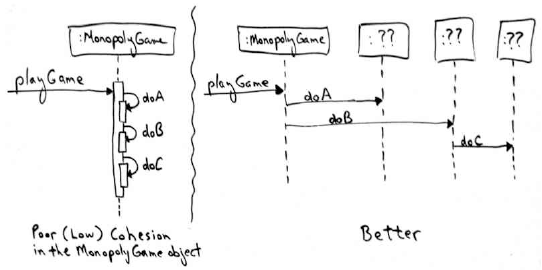
\includegraphics{Immagini/Schermata_20260712_184505.png}
\end{figure}

\subsection{Esempio MonopoluGame}
\begin{figure}[H]
    \centering
    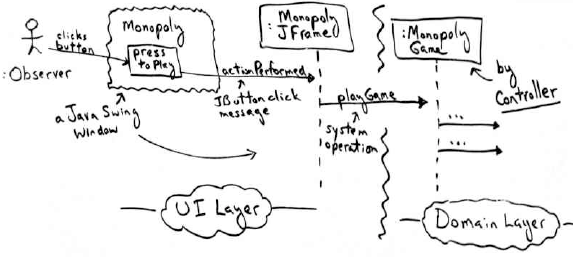
\includegraphics{Immagini/Schermata_20260712_184418.png}
\end{figure}

\newpage
\section{High Cohesion}
\subsection{Definizione}
\begin{table}[htbp]
    \renewcommand{\arraystretch}{1.8}
    \begin{tabularx}{\textwidth}{@{} p{2.8cm} X @{}}
        \hline
        Nome: & \textbf{High Cohesion} \\
        \hline
        Problema: &  Come mantenere gli oggetti focalizzati, comprensibili e gestibili e, come effetto collaterale, sostenere Low Coupling?\\
        \hline
        Soluzione : &
        Assegna le responsabilità in modo tale che la coesione rimanga alta.

        Usa questo principio per valutare le alternative
        \\
        \hline
    \end{tabularx}
\end{table}

\chapter{Patter GRASP Avanzati}
\section{Pure Fabricator}
\subsection{Definizione}
\begin{table}[htbp]
    \renewcommand{\arraystretch}{1.8}
    \begin{tabularx}{\textwidth}{@{} p{2.8cm} X @{}}
        \hline
        Nome: & \textbf{Pure Fabricator} \\
        \hline
        Problema: &  Quale oggetto deve avere la responsabilità quando non si vogliono violare High Cohesion e Low Coupling, o altri obiettivi, ma le soluzioni suggerite da Expert non sono appropriate?\\
        \hline
        Soluzione : &
        Assegnare un insieme di responsabilità altamente coeso a una classe artificiale o di convenienza, che non rappresenta un concetto del dominio del problema, ma piuttosto è una classe inventata per sostenere coesione alta, accoppiamento basso e riuso
        \\
        \hline
    \end{tabularx}
\end{table}

\subsection{Esempio POS NextGen}
Vogliamo salvare l'oggetto di tipo Sale in una base di dati razionale.

Solitamente questa responsabilità è assegnata alla classe stessa, ma Sale perderebbe di prestazioni:
\begin{itemize}
    \item Meno coesione perchè introduciamo le operazioni orientate ai db
    \item Aumento dell'accoppiamento all'interfaccia del db
    \item Diminuirebbe il riuso futuro della classe stessa
    \item Possibile codice duplicato con altre classi
\end{itemize}

\begin{figure}[H]
    \centering
    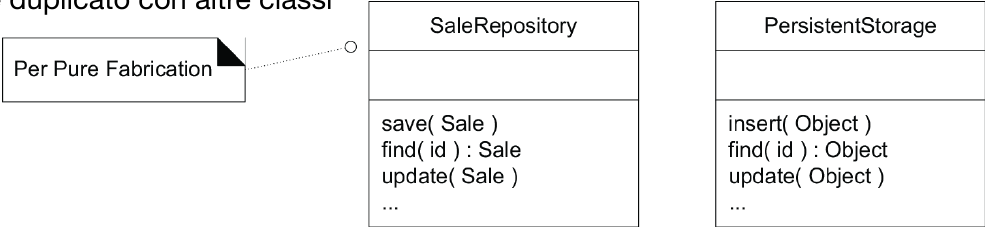
\includegraphics[scale=0.7]{Immagini/Schermata_20260712_185607.png}
\end{figure}

\newpage
\section{Polymorphism}
\subsection{Definizione}
\begin{table}[htbp]
    \renewcommand{\arraystretch}{1.8}
    \begin{tabularx}{\textwidth}{@{} p{2.8cm} X @{}}
        \hline
        Nome: & \textbf{Polymorphism} \\
        \hline
        Problema: &  Come gestire alternative basate sul tipo?
        
        Come creare componenti software inseribili?
        \\
        \hline
        Soluzione : &
        Quando le alternative e comportamenti correlati variano con il tipo, allora assegna la responsabilità del comportamento ai tipi per i quali il comportamente varia, utilizzando operazione polimorfe
        \\
        \hline
    \end{tabularx}
\end{table}

\subsection{Esempio POS NextGen}
Vogliamo gestire i diversi sistemi di contabilità di terze parti.

Dobbiamo far sì che il sistema di contabilità di POS NextGen possa comunicare con loro.

Così facendo abbiamo più implementazioni simili ma che si adattano a differenti richieste

\begin{figure}[H]
    \centering
    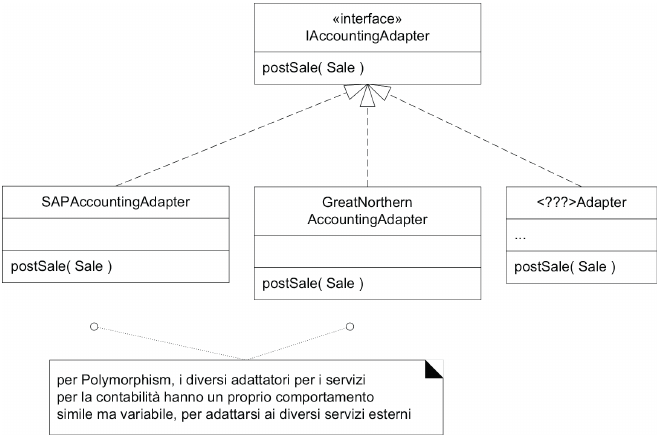
\includegraphics[scale=0.6]{Immagini/Schermata_20260712_185958.png}
\end{figure}

\subsection{Esempio Monopoly}
Nel gioco del Monopolu le caselle possono avere un comportamento differente in base al loro tipo, anche se condividono delle caratteristiche comuni

\begin{figure}[H]
    \centering
    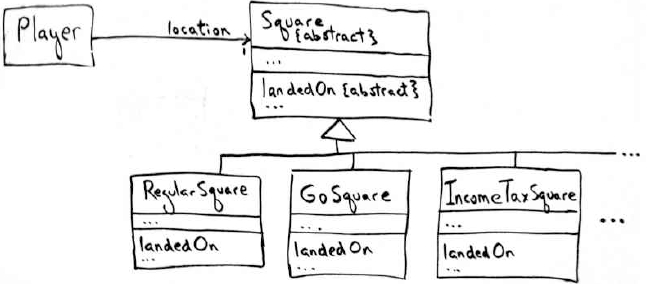
\includegraphics[scale=0.6]{Immagini/Schermata_20260712_190147.png}
\end{figure}

\newpage
\section{Indirection}
\subsection{Definizione}
\begin{table}[htbp]
    \renewcommand{\arraystretch}{1.8}
    \begin{tabularx}{\textwidth}{@{} p{2.8cm} X @{}}
        \hline
        Nome: & \textbf{Indirection} \\
        \hline
        Problema: &  Dove assengare una responsabilità, per evitare l'accoppiamento diretto tra più elementi?

        Come disaccoppiare gli oggetti in modo da sostenere un alto riuso e un accoppiamento basso?
        \\
        \hline
        Soluzione : &
        Si assegna la responsabilità ad un oggetto intermediario che media tra altri componenti o servizi, in modo che non ci sia un accoppiamento diretto tra di essi
        \begin{itemize}
            \item L'intermediario crea una indirezione tra le componenti
            \item Accoppiamento più basso tra componenti
        \end{itemize}
        \\
        \hline
    \end{tabularx}
\end{table}

\subsection{Esempio POS NextGen}
\begin{itemize}
    \item Gli oggetti lAccountingAdapter fungono da intermediari tra gli oggetti dello strato di dominio e i servizi esterni
    \item Aggiungendo un livello di indicazione e il polimorfismo gli oggetti adattatori proteggono il progetto interno da variazione nelle interfacce esterne
\end{itemize}
\begin{figure}[H]
    \centering
    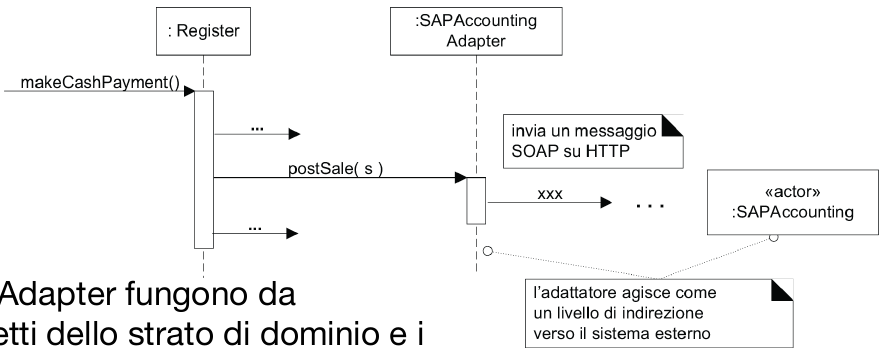
\includegraphics[scale=0.8]{Immagini/Schermata_20260712_190717.png}
\end{figure}

\newpage
\section{Protected Variations}
\subsection{Definizione}
\begin{table}[htbp]
    \renewcommand{\arraystretch}{1.8}
    \begin{tabularx}{\textwidth}{@{} p{2.8cm} X @{}}
        \hline
        Nome: & \textbf{Protected Variations} \\
        \hline
        Problema: &  Come progettare oggetti, sottosistemi e sistemi in modo tale che le variazioni o l'instabilità di questi elementi non si riversino su altri elementi?\\
        \hline
        Soluzione : &
        Si identificano i punti in cui sono previste delle variazioni, poi si assegnano le responsabilità per creare una "interfaccia" stabile attorno a questi punti
        \\
        \hline
    \end{tabularx}
\end{table}